\documentclass[sigconf, nonacm]{acmart}
\usepackage{pvldb}
\usepackage{booktabs}
\usepackage{multirow}
\usepackage{pifont}
\usepackage[ruled,vlined,linesnumbered]{algorithm2e}
\renewcommand\vldbdoi{XX.XX/XXX.XX}
\renewcommand\vldbpages{XXX-XXX}
\renewcommand\vldbavailabilityurl{}
\graphicspath{{../../figures/}}
\emergencystretch=1.5em

\newtheorem{theorem}{Theorem}
\newtheorem{proposition}{Proposition}
\newtheorem{lemma}{Lemma}
\newtheorem{definition}{Definition}

\newcommand{\cmark}{\ding{51}}
\newcommand{\xmark}{\ding{55}}
\newcommand{\pmark}{$\triangle$}

\begin{document}
\title{StratQ: Anytime-Valid Grouped Query Contracts for Expensive Predicates}
\author{Author information pending}

\begin{abstract}
Analytical SQL queries over text, images, and structured records increasingly evaluate expensive neural or language-model predicates inside \texttt{GROUP BY} count, \texttt{HAVING}, and top-$k$ operators.
Evaluating the reference model on every row dominates query latency, yet existing proxy-assisted and approximate query engines typically protect only an overall aggregate, assume fixed sample sizes or large-sample asymptotics, or omit decision certification under early stopping.
We present \textsc{StratQ}, a query execution engine and statistical contract for fixed-snapshot grouped queries with expensive binary predicates.
Under uniform sampling without replacement within each adaptively selected group, \textsc{StratQ} couples remaining-population centering with a predictable, analytically cross-validated Ridge control variate that reverts to a zero-range baseline unless its leave-one-out cost surrogate improves by at least 5\%.
All group intervals are computed via directed binary64 outward rounding and share a single $(1-\delta)$ simultaneous coverage event across all groups and data-dependent reveal times, directly certifying \texttt{COUNT} tolerances, \texttt{HAVING} thresholds, and top-$k$ membership while permitting explicit abstention under budget caps.
Implemented over DuckDB and Apache Arrow and evaluated across six workload families (including live GPU DistilBERT-SST2 and ResNet34-224 inference and 10M-row Parquet snapshots) and eleven database/modern operator adaptations plus an independent grouped hypergeometric CS, \textsc{StratQ} delivers $3.61\times$--$4.78\times$ ratio-of-medians query-level GPU speedups after proxy scoring, certifies top-2 membership on Yelp with $3.0\%$ of rows ($6.5\times$ fewer calls than raw stratified WoR), observes $30/30$ all-group coverage over 15 skewed Zipf configurations (two seeds each) versus $0/30$ for a global-count surrogate's group plugs and $16/30$ for an optional-stopping CLT diagnostic, and records an 85.6\,MB query-stage traced-allocation peak at 10M rows.
\end{abstract}

\maketitle
\vldbtopmatter

\section{Introduction}
\label{sec:intro}

Modern data-management workloads routinely pair relational grouping with expensive machine-learning or large-language-model (LLM) predicates~\cite{kang2019blazeit,patel2025lotus,liu2025palimpzest,shankar2025docetl}.
Consider a content-moderation or product-analytics query over a fixed Parquet snapshot:
\begin{quote}\small\ttfamily
SELECT category, COUNT(*) AS pos\_cnt FROM items\\
WHERE REF\_MODEL(content) = 1 GROUP BY category\\
HAVING pos\_cnt >= 2178 \quad\textnormal{(or ORDER BY pos\_cnt DESC LIMIT 2)}
\end{quote}
When \texttt{REF\_MODEL} is a Transformer or vision network executing on a GPU, running an exhaustive pass over tens of thousands of rows takes tens of seconds to minutes.
Analysts therefore rely on cheap proxies---such as TF-IDF classifiers, thumbnail regressors, or structured metadata---and adaptive sampling to avoid evaluating the reference model on every tuple~\cite{kang2017noscope,kang2020supg,kang2021abae,zeighami2026bargain}.

Despite rapid progress in approximate query processing (AQP) and semantic query engines, a critical gap remains between \emph{approximate execution} and \emph{certifiable grouped SQL semantics}.
Specifically, three failure modes arise when existing systems are applied to grouped analytical queries with expensive predicates:
\begin{enumerate}
  \item \textbf{Silent per-group collapse under global guarantees.} Systems such as SUPG~\cite{kang2020supg} and BARGAIN~\cite{zeighami2026bargain} control an \emph{overall} accuracy, precision, or recall target. Such a contract does not imply a per-group count guarantee under skewed sizes or heterogeneous prevalences. In our 100K-row Zipf stress suite (\S\ref{sec:eval-systems}), a global-count surrogate's proportional group intervals cover all groups in $0/30$ trials and cover $0\%$ of tail groups; this is not a failure of BARGAIN's original global guarantee.
  \item \textbf{Coverage breakdown under optional stopping and small groups.} Classical grouped AQP~\cite{acharya2000congress,park2018verdict,walenz2019lws} and database-agnostic simultaneous-error engines such as PilotDB~\cite{zhu2025pilotdb} rely on fixed-look allocations or central limit theorem (CLT) asymptotics. PilotDB excludes aggregates used as \texttt{GROUP BY} keys (e.g., \texttt{GROUP BY COUNT(*)}), not ordinary \texttt{COUNT} outputs. Reusing its fixed-look CLT intervals at data-dependent looks does not guarantee nominal coverage and can be anti-conservative: in our optional-stopping diagnostic, the asymptotic comparator drops to $16/30$ all-group coverage overall and $0/6$ at $G=100$.
  \item \textbf{Range-penalty degradation under weak proxies and uncertified floating-point endpoints.} Using a cheap proxy as a control variate~\cite{kang2019blazeit,angelopoulos2023ppi,zhou2026celeus} reduces variance when the proxy is accurate, but finite-sample empirical-Bernstein and betting bounds also scale with the prediction range $R_s = 1 + f_{\max} - f_{\min}$. When a proxy is weak or noisy, an unguarded control variate can increase reference calls relative to sampling without a proxy. Moreover, real-arithmetic confidence sequences can silently lose validity in IEEE-754 binary64 arithmetic at census ties or tight endpoints.
\end{enumerate}

\paragraph{Positioning against concurrent 2025--2026 work}
Recent statistical and database papers occupy several individual pieces of this space, and we delimit our scope explicitly rather than claiming isolated statistical components as new.
Waudby-Smith and Ramdas~\cite{wor2020,waudby2024betting} establish finite-population without-replacement (WoR) empirical-Bernstein betting confidence sequences (CS).
Spertus et al.~\cite{spertus2026sequential} combine predictable cross-stratum selection, WoR remaining-population means, and simultaneous lower confidence bounds.
Hait~\cite{hait2026target} develops adaptive cross-group allocation and multi-target anytime certification under i.i.d.\ within-stratum observations.
CELEUS~\cite{zhou2026celeus} constructs finite-pool WoR anytime intervals with fixed surrogate completion and e-process inversion; as we show in Proposition~\ref{prop:celeus-equiv}, its uniform-WoR fixed-proxy signal shares the exact same finite-population identity as a fixed-predictor specialization of our observation.
Meanwhile, PilotDB~\cite{zhu2025pilotdb} formalizes simultaneous multi-group relative error in SQL (asymptotically, fixed-look), and BARGAIN~\cite{zeighami2026bargain} applies anytime-valid inference to global LLM cascades.

\paragraph{Core thesis and contributions}
\textsc{StratQ} does not claim a new concentration inequality, nor does it claim that a proxy always accelerates every query.
Instead, its contribution is an \emph{end-to-end, database-facing grouped query contract and execution engine} that unifies predictable batch-refitted residual control variates, uniform within-group WoR sampling, cross-group adaptive routing, and directed binary64 outward rounding under a single filtration and $(1-\delta)$ joint coverage event.
To our knowledge across 2020--2026 literature in WoR confidence sequences, prediction-powered inference, stratified sequential inference, and semantic query systems, no prior system combines all of these guarantees into a single SQL execution contract for \texttt{COUNT}, \texttt{HAVING}, and \texttt{TOP-$k$} with explicit abstention (Table~\ref{tab:contract-matrix}).
We make four concrete contributions:
\begin{itemize}
  \item \textbf{Certified grouped query contract (\S\ref{sec:contract}).} We formalize fixed-snapshot grouped \texttt{COUNT}, \texttt{HAVING}, and \texttt{TOP-$k$} semantics over known group keys and binary reference outputs, including empty-positive-count groups, explicit budget-cap abstention, and deterministic tie-breaking at census.
  \item \textbf{Predictable Safe-LOO control variates and outward-rounded CS (\S\ref{sec:method}).} We prove simultaneous anytime validity under cross-group adaptive routing and batch-refitted predictors (Theorem~\ref{thm:coverage}), design an analytic Ridge leave-one-out (LOO) range--variance gate that reverts to a zero-range baseline unless its predicted betting cost improves by at least 5\%, and establish a directed binary64 outward-rounding implementation whose empty-intersection restarts are provably restricted to the complement of the coverage event (Theorem~\ref{thm:fp}).
  \item \textbf{DuckDB and Apache Arrow execution engine (\S\ref{sec:system}).} We build a reusable columnar profiling and zero-copy Arrow transfer pipeline with directed feature-sum envelopes, three query-specific routing policies, and microsecond-scale scalar directed-rounding arithmetic ($36.6\times$ faster than naive NumPy array-dispatched enclosures).
  \item \textbf{Comprehensive real-GPU and systems evaluation (\S\ref{sec:eval}).} Across six workload families---including live GPU DistilBERT-SST2 (20K Yelp reviews) and ResNet34-224 (10K CIFAR-10 images), UCI Adult, SMS Spam, Fashion-MNIST, and synthetic Parquet scale/stress---and eleven database/modern operator adaptations plus an independent grouped hypergeometric CS, we separate reference calls, certification rates, cold/warm latency amortization, and isolated-subprocess memory attribution, while transparently reporting weak-proxy and low-within-group-variance boundary regimes.
\end{itemize}

\begin{table*}[t]
\centering
\footnotesize
\setlength{\tabcolsep}{4pt}
\caption{Contract comparison between \textsc{StratQ} and related database/statistical approaches (2019--2026). This is a capability matrix, not a benchmark of full system replicas. \cmark\ denotes support in the stated main contract, \pmark\ partial/variant/asymptotic overlap, and \xmark\ unsupported. ``Batch-refit CV'' means predictable row-level residual control-variate refitting; ``route'' means cross-group routing; ``SQL cert.'' means certified grouped \texttt{HAVING}/\texttt{TOP-$k$}.}
\label{tab:contract-matrix}
\begin{tabular}{@{}lccccccc@{}}
\toprule
System / Method & Fixed-pop. WoR & Finite anytime & Batch-refit CV & Cross-group route & Per-group count CI & SQL decision cert. & DB execution \\
\midrule
BlazeIt~\cite{kang2019blazeit} (PVLDB'19) & \xmark & \cmark & \pmark & \xmark & \xmark & \pmark & \cmark \\
ABae~\cite{kang2021abae} (PVLDB'21) & \cmark & \xmark & \xmark & \pmark & \pmark & \xmark & \pmark \\
LOTUS~\cite{patel2025lotus} (PVLDB'25) & \xmark & \xmark & \xmark & \pmark & \pmark & \pmark & \cmark \\
PilotDB~\cite{zhu2025pilotdb} (SIGMOD'25) & \pmark & \xmark\ (CLT) & \xmark & \pmark & \pmark & \xmark & \cmark \\
BARGAIN~\cite{zeighami2026bargain} (PACMMOD'25) & \pmark & \cmark & \xmark & \xmark & \xmark\ (global) & \xmark & \xmark \\
Spertus et al.~\cite{spertus2026sequential} (arXiv'26) & \cmark & \cmark & \xmark & \cmark & \pmark\ (LCB) & \xmark & \xmark \\
Hait~\cite{hait2026target} (arXiv'26) & \xmark\ (i.i.d.) & \cmark & \xmark & \cmark & \pmark & \xmark & \xmark \\
CELEUS~\cite{zhou2026celeus} (arXiv'26) & \cmark & \cmark & \xmark\ (fixed) & \xmark\ (single) & \xmark & \xmark & \xmark \\
\midrule
\textbf{\textsc{StratQ} (this work)} & \cmark & \cmark\ (+FP64) & \cmark & \cmark & \cmark & \cmark\ (+abstain) & \cmark\ (DuckDB+Arrow) \\
\bottomrule
\end{tabular}
\end{table*}

\section{Query Contract and Semantics}
\label{sec:contract}

We formalize the fixed-snapshot SQL query semantics enforced by the \textsc{StratQ} execution API.

\paragraph{Fixed snapshot and group universe}
A query operates over a static relational table snapshot $T$ containing $N$ rows with known, inexpensive grouping keys $g(i) \in \mathcal{G}$ (where $|\mathcal{G}| = G \ge 1$) and cheap feature vectors $\phi_i \in [0, 1]^d$ (typically an intercept $1$, a normalized proxy score, and optional relational covariates from Parquet columns).
Each row $i \in \{1,\dots,N\}$ carries an unknown, deterministic binary reference predicate value $y_i \in \{0, 1\}$ produced by an expensive callback $\mathcal{O}(i)$ (e.g., a GPU neural classifier or LLM judge).
Let $I_g = \{i \in \{1,\dots,N\} : g(i) = g\}$ denote the nonempty row-index set of group $g$, with known cardinality $N_g = |I_g| \ge 1$ and $\sum_{g \in \mathcal{G}} N_g = N$.
The unknown target for group $g$ is the exact reference-positive count and positive rate:
\begin{equation}
  K_g = \sum_{i \in I_g} y_i \in \{0, 1, \dots, N_g\}, \qquad \mu_g = \frac{K_g}{N_g} \in [0, 1].
\end{equation}
The reported universe $\mathcal{G}$ includes every nonempty input group, including groups with $K_g = 0$, matching SQL \texttt{SUM(CAST(REF\_MODEL(x) AS INT)) GROUP BY g} semantics.

\paragraph{Joint anytime coverage contract}
The analyst specifies a query-level failure probability $\delta \in (0, 1)$ and an optional reference-call budget cap $B_{\max} \le N$.
At every global reveal step $t \in \{0, 1, \dots, N\}$ at which the engine evaluates the reference model on one more row, \textsc{StratQ} maintains count intervals $[L_g(t), U_g(t)] \subseteq [0, N_g]$ for all $g \in \mathcal{G}$.
The engine guarantees the single simultaneous coverage event:
\begin{align}
  \mathcal{E} &:= \bigl\{\forall\, t \in \{0,\dots,N\},\; \forall\, g \in \mathcal{G}:\; L_g(t) \le K_g \le U_g(t)\bigr\}, \nonumber\\
  \Pr(\mathcal{E}) &\ge 1 - \delta.
  \label{eq:joint-event}
\end{align}
Because $\mathcal{E}$ holds uniformly over all reveal times $t$ and all groups $g$, the query engine may inspect intervals after every batch, adaptively redirect oracle calls to unresolved groups, and terminate at any data-dependent stopping time $\tau \le B_{\max}$ without invalidating coverage or spending extra failure budget per look.

\paragraph{Three certified SQL query modes}
All three analytical query operators inherit their correctness directly from the single event $\mathcal{E}$:
\begin{itemize}
  \item \textbf{Grouped \texttt{COUNT} with per-group tolerances.} The analyst supplies per-group absolute tolerances $\epsilon_g \ge 0$ (e.g., $\epsilon_g = 0.04 N_g$). The engine returns $[L_g(\tau), U_g(\tau)]$ and midpoint $\hat{K}_g = \tfrac{1}{2}(L_g(\tau)+U_g(\tau))$, stopping once $\tfrac{1}{2}(U_g(\tau)-L_g(\tau)) \le \epsilon_g$ for every $g \in \mathcal{G}$ or when $\tau = B_{\max}$. On $\mathcal{E}$, $|\hat{K}_g - K_g| \le \tfrac{1}{2}(U_g(\tau)-L_g(\tau))$ simultaneously for all $g$; if stopped early by $B_{\max}$, the engine reports realized half-widths honestly alongside a \texttt{converged=false} flag.
  \item \textbf{Grouped \texttt{HAVING} ($K_g \ge \tau_{\text{cnt}}$).} Given threshold $\tau_{\text{cnt}}$, \textsc{StratQ} partitions $\mathcal{G}$ into accepted groups $\{g : L_g(\tau) \ge \tau_{\text{cnt}}\}$, rejected groups $\{g : U_g(\tau) < \tau_{\text{cnt}}\}$, and explicitly \emph{unresolved} (abstained) groups whose interval still straddles $\tau_{\text{cnt}}$. On $\mathcal{E}$, every accepted and rejected label is exact; under a tight budget $B_{\max}$, borderline groups abstain rather than guessing.
  \item \textbf{Grouped \texttt{TOP-$k$} ($0 < k < G$).} A candidate $k$-element subset $A \subset \mathcal{G}$ is certified if and only if
  \begin{equation}
    \min_{g \in A} L_g(\tau) \;>\; \max_{h \notin A} U_h(\tau).
    \label{eq:topk-cert}
  \end{equation}
  On $\mathcal{E}$, strict separation guarantees exact top-$k$ set membership. When exact ties occur ($K_{(k)} = K_{(k+1)}$), strict separation is impossible prior to census; \textsc{StratQ} refuses premature certification, abstains under insufficient budget, and resolves exact ties deterministically by secondary group-key order only once the tied boundary groups reach full census ($t_g = N_g$).
\end{itemize}

\paragraph{Contract boundaries}
Equation~\eqref{eq:joint-event} governs fidelity to the deterministic reference model $\mathcal{O}$ on the fixed snapshot $T$, independent of $\mathcal{O}$'s external accuracy on human ground truth. Each query receives its own risk budget $\delta$; cross-query risk reuse, streaming table mutations, and unknown group keys lie outside the current contract and are discussed in \S\ref{sec:limitations}.

\section{Statistical Foundations and Directed-Rounding Safety}
\label{sec:method}

We now present the mathematical construction underlying \textsc{StratQ}: the proxy-adjusted WoR observation, the simultaneous anytime-valid confidence sequence under cross-group routing, its exact algebraic relationship to fixed-proxy finite-pool inference, the analytic Ridge LOO range--variance gate, and the directed binary64 outward-rounding enclosure.

\subsection{Filtration and Proxy-Adjusted WoR Observation}
\label{sec:wor-obs}

Fix the snapshot labels $\{y_i\}_{i=1}^N$ and group partition $\{I_g\}_{g \in \mathcal{G}}$.
Let $\mathcal{F}_{t-1}$ be the $\sigma$-algebra generated by all cheap features $\{\phi_i\}_{i=1}^N$, group keys, and all reference labels and routing choices revealed strictly before global reveal step $t$.
At global step $t$, the scheduler selects an active, non-exhausted group $g_t \in \mathcal{G}$ as an $\mathcal{F}_{t-1}$-measurable random variable.
Conditional on $\mathcal{F}_{t-1}$ and $g_t = g$, the next revealed row $i_t$ is drawn uniformly at random without replacement from the unrevealed rows $I_g^{\text{rem}}$ of group $g$.
In execution, pre-generating an independent uniform random permutation of each $I_g$ implements this reveal law identically, provided the scheduler and predictor never inspect unrevealed suffix indices or labels.

Suppressing the group index $g$, consider local reveal step $s \in \{1, \dots, N\}$ of a group of size $N$ with unknown mean $\mu = K/N$.
Before draw $s$, let $m_s = N - s + 1$ be the remaining group size, $w_s = N / m_s$, and $h_s = S_{s-1} / m_s$, where $S_{s-1} = \sum_{r=1}^{s-1} y_{i_r}$ is the sum of already revealed labels.
Let $f_s : I_g \to \mathbb{R}$ be any $\mathcal{F}_{t-1}$-predictable function of the cheap features, with known remaining-population mean $\bar{f}_s = \frac{1}{m_s}\sum_{j \in I_g^{\text{rem}}} f_s(j)$ and valid predictable bounds $f_{\min,s} \le f_s(j) \le f_{\max,s}$ for all $j \in I_g^{\text{rem}}$.
For the revealed row $i_s$, define
\begin{align}
  Z_s &= \bar{f}_s + y_{i_s} - f_s(i_s), &
  a_s &= \bar{f}_s - f_{\max,s}, \label{eq:z-def}\\
  R_s &= 1 + f_{\max,s} - f_{\min,s}, &
  X_s &= \frac{Z_s - a_s}{R_s}. \label{eq:x-def}
\end{align}
Because $y_{i_s} \in [0, 1]$ and $f_s(i_s) \in [f_{\min,s}, f_{\max,s}]$, we have $Z_s \in [a_s, a_s + R_s]$ and therefore $X_s \in [0, 1]$ almost surely.
By conditional uniformity of $i_s$ over $I_g^{\text{rem}}$, $\mathbb{E}[f_s(i_s) \mid \mathcal{F}_{t-1}, g_t = g] = \bar{f}_s$, so the two predictor terms cancel identically in conditional expectation:
\begin{align}
  \mathbb{E}[Z_s \mid \mathcal{F}_{t-1}, g_t = g] &= \frac{K - S_{s-1}}{m_s} = w_s \mu - h_s, \nonumber\\
  \eta_s := \mathbb{E}[X_s \mid \mathcal{F}_{t-1}, g_t = g] &= \frac{w_s \mu - h_s - a_s}{R_s}.
  \label{eq:cond-mean}
\end{align}
When $f_s$ is constant across the group (the no-proxy baseline), $f_{\max,s} = f_{\min,s}$, $Z_s = y_{i_s}$, $R_s = 1$, and $X_s = y_{i_s}$.

\subsection{Simultaneous Confidence Sequence under Adaptive Routing}
\label{sec:cs-theorem}

Following the predictable empirical-Bernstein betting framework of Waudby-Smith and Ramdas~\cite{wor2020,waudby2024betting}, at each local step $s$ choose an $\mathcal{F}_{t-1}$-predictable center $p_s \in [0, 1]$ and betting parameter $\lambda_s \in [0, 1)$, and write $\psi(\lambda) = -\log(1 - \lambda) - \lambda$.
Maintain three running accumulators per group after $t_g$ local reveals:
\begin{align}
  A_{t_g} &= \sum_{s=1}^{t_g} \frac{\lambda_s w_s}{R_s}, &
  B_{t_g} &= \sum_{s=1}^{t_g} \frac{\lambda_s (Z_s + h_s)}{R_s}, \nonumber\\
  V_{t_g} &= \sum_{s=1}^{t_g} \psi(\lambda_s)(X_s - p_s)^2.
  \label{eq:accum}
\end{align}
Assign each group a positive risk budget $\alpha_g > 0$ satisfying $\sum_{g \in \mathcal{G}} \alpha_g \le \delta$ (default uniform $\alpha_g = \delta / G$), and set $b_{t_g} = V_{t_g} + \log(2 / \alpha_g)$.
When $A_{t_g} > 0$, define the raw statistical interval
\begin{equation}
  J_g(t_g) = \left[\frac{B_{t_g} - b_{t_g}}{A_{t_g}},\; \frac{B_{t_g} + b_{t_g}}{A_{t_g}}\right],
\end{equation}
and $J_g(t_g) = (-\infty, +\infty)$ when $A_{t_g} = 0$.
Let $D_g(t_g) = [S_{t_g}/N_g,\; (S_{t_g} + N_g - t_g)/N_g]$ be the exact deterministic feasibility interval.
Initializing $I_g(0) = [0, 1]$, update $I_g(t_g) = I_g(t_g - 1) \cap J_g(t_g) \cap D_g(t_g)$. In real arithmetic this intersection is nonempty on the coverage event. In safe mode, restart to $D_g(t_g)$ only when the conservative previous and deterministic intervals are disjoint; if only the conservative three-way intersection is empty, report the convex hull of the three enclosures. At census $t_g = N_g$, $D_g(N_g) = \{\mu_g\}$ is exact. Scale by $N_g$ to produce $[L_g, U_g] = [N_g \min I_g, N_g \max I_g]$.

\begin{theorem}[Simultaneous Anytime Grouped Coverage]
\label{thm:coverage}
Under the fixed-snapshot conditional uniformity and $\mathcal{F}_{t-1}$-predictability conditions above, if $\alpha_g > 0$ for all $g \in \mathcal{G}$ and $\sum_{g \in \mathcal{G}} \alpha_g \le \delta$, then the count intervals $[L_g(t), U_g(t)]$ satisfy Eq.~\eqref{eq:joint-event}: $\Pr(\mathcal{E}) \ge 1 - \delta$.
\end{theorem}

\begin{proof}
For any $|x| \le 1$ and $\lambda \in (0, 1)$, let $u = \lambda x$. Integration by parts yields
\[
  u - \log(1 + u) = u^2 \int_0^1 \frac{r}{1 + u r}\,dr \le u^2 \int_0^1 \frac{r}{1 - \lambda r}\,dr = x^2 \psi(\lambda),
\]
because $r/(1+ur)$ is decreasing in $u \ge -\lambda$.
Rearranging gives $\exp(u - x^2 \psi(\lambda)) \le 1 + u$.
For either sign $\sigma \in \{-1, +1\}$, set $x = \sigma(X_s - p_s) \in [-1, 1]$ and $v = \sigma \lambda_s (\eta_s - p_s)$.
Since $\sigma \lambda_s(X_s - \eta_s) = \sigma \lambda_s(X_s - p_s) - v$, conditioning on $(\mathcal{F}_{t-1}, g_t = g)$ gives
\begin{align*}
  \mathbb{E}\!\left[\exp\!\bigl\{\sigma \lambda_s(X_s - \eta_s) - \psi(\lambda_s)(X_s - p_s)^2\bigr\} \,\middle|\, \mathcal{F}_{t-1}, g_t=g\right] \\
  \le e^{-v}\bigl(1 + \sigma \lambda_s \mathbb{E}[X_s - p_s \mid \mathcal{F}_{t-1}, g_t=g]\bigr) = e^{-v}(1 + v) \le 1.
\end{align*}
At $\lambda_s = 0$ the factor equals $1$.
Now fix group $g$ and sign $\sigma$, and define the global process $M_g^{(\sigma)}(0) = 1$ with step multiplier $E_{g,t}^{(\sigma)}$ equal to the exponential factor above when $g_t = g$, and equal to $1$ when $g_t \ne g$.
Because $g_t$ is $\mathcal{F}_{t-1}$-measurable, the tower property yields $\mathbb{E}[M_g^{(\sigma)}(t) \mid \mathcal{F}_{t-1}] \le M_g^{(\sigma)}(t-1)$, so $M_g^{(\sigma)}$ is a nonnegative supermartingale with respect to the \emph{single global filtration} $\{\mathcal{F}_t\}_{t \ge 0}$.
Expanding Eq.~\eqref{eq:x-def}--\eqref{eq:cond-mean} shows that $X_s - \eta_s = (Z_s + h_s - w_s \mu_g)/R_s$, so at local count $t_g$ the log supermartingale equals $\log M_g^{(\sigma)}(t) = \sigma(B_{t_g} - A_{t_g}\mu_g) - V_{t_g}$.
By Ville's maximal inequality, $\Pr(\exists t : M_g^{(\sigma)}(t) \ge 2/\alpha_g) \le \alpha_g/2$.
A union bound over $\sigma \in \{-1,+1\}$ and $g \in \mathcal{G}$ ensures that with probability at least $1 - \sum_g \alpha_g \ge 1 - \delta$, $\mu_g \in J_g(t_g)$ holds for all $g$ and all $t$.
Since $\mu_g \in D_g(t_g)$ deterministically at every step, intersecting $I_g(t_g-1)$, $J_g(t_g)$, and $D_g(t_g)$ preserves $\mu_g \in I_g(t_g)$ (and never produces an empty intersection) throughout this event.
\end{proof}

\paragraph{Exact algebraic relation to CELEUS and fixed-proxy PPI}
To position Theorem~\ref{thm:coverage} honestly against recent finite-pool prediction-assisted work~\cite{angelopoulos2023ppi,zhou2026celeus}, we record the exact equivalence in the fixed-predictor special case.

\begin{proposition}[Fixed-Proxy Identity vs.\ Batch Refitting]
\label{prop:celeus-equiv}
Suppose $f_s \equiv f$ is fixed across all draws in a single group of size $N$.
(i) Defining residuals $r_i = y_i - f(i)$ with group sum $F = \sum_{i \in I_g} f(i)$ and seen sum $F_{s-1}$, we have $Z_s = \bar{f}_s + r_{i_s}$ and $\mathbb{E}[Z_s \mid \mathcal{F}_{t-1}] = (K - S_{s-1})/m_s = (F - F_{s-1})/m_s + \mathbb{E}[r_{i_s} \mid \mathcal{F}_{t-1}]$, which is algebraically identical to centering a fixed-residual population~\cite{angelopoulos2023ppi}.
(ii) Under uniform WoR sampling ($q_s = 1/m_s$), CELEUS's surrogate-completed IPW signal~\cite{zhou2026celeus} satisfies $\hat{S}_s = (S_{s-1} + m_s \bar{f}_s)/N + m_s (y_{i_s} - f(i_s))/N = (S_{s-1} + m_s Z_s)/N$, giving $\mathbb{E}[\hat{S}_s \mid \mathcal{F}_{t-1}] = \mu$ via the exact same remaining-population identity.
\end{proposition}

Proposition~\ref{prop:celeus-equiv} clarifies that the term ``remaining-population centering'' is \emph{not} a novel estimator for a fixed predictor.
Rather, the value of Eq.~\eqref{eq:z-def}--\eqref{eq:accum} lies in combining four properties inside one global filtration: (1) $f_s$ may be refitted between batches using prior labels without breaking Eq.~\eqref{eq:cond-mean}; (2) uniform within-group WoR avoids IPW variance blowup when proxy scores are weak or uncalibrated; (3) one global supermartingale collection covers all $G$ groups simultaneously under adaptive cross-group routing; and (4) the resulting count intervals certify \texttt{HAVING} and \texttt{TOP-$k$} decisions directly.

\subsection{Predictable Safe-LOO Range--Variance Gating}
\label{sec:safe-loo}

A subtle pitfall of prediction-assisted betting intervals is the tension between \emph{residual variance} and \emph{prediction range}.
In Eq.~\eqref{eq:accum}, reducing $\mathrm{Var}(y_i - f_s(i))$ shrinks $V_{t_g}$, but any non-constant predictor expands the range factor from $R_0 = 1$ to $R_s = 1 + f_{\max,s} - f_{\min,s} > 1$, which shrinks $A_{t_g} \propto 1/R_s$ and inflates the threshold term $\log(2/\alpha_g)/A_{t_g}$.
Consequently, fitting a noisy proxy on a small sample of group labels---or evaluating it with optimistic in-sample residual variance---can \emph{increase} reference calls compared to disabling the proxy entirely.

To guard against weak-proxy degradation while strictly preserving $\mathcal F_{t-1}$-predictability, \textsc{StratQ} introduces an analytic Ridge leave-one-out (LOO) range--variance gate (\texttt{safe\_loo}) executed before each batch using only previously revealed labels in group $g$ ($n_g$ rows) and a periodically refreshed pooled ridge predictor $\theta_{\text{global}}$.
Let $r = y_{\text{seen}} - \Phi_{\text{seen}} \theta_{\text{global}}$ be the prior residuals and center both $r$ and the non-intercept feature columns $\Phi_c$.
For each shrinkage candidate $\kappa \in \mathcal{K} = \{0, 0.1, 0.25, 0.5, 0.75, 1.0\}$, form $Z_\kappa = \kappa \Phi_c$ and fit the Ridge correction with penalty $\Lambda = \lambda_{\text{ridge}} I$:
\begin{equation}
  \beta_\kappa = (Z_\kappa^\top Z_\kappa + \Lambda)^{-1} Z_\kappa^\top (r - \bar{r}\mathbf{1}), \quad
  H_\kappa = \frac{\mathbf{1}\mathbf{1}^\top}{n_g} + Z_\kappa (Z_\kappa^\top Z_\kappa + \Lambda)^{-1} Z_\kappa^\top.
  \label{eq:ridge-hat}
\end{equation}
Using the hat-matrix diagonal $h_{ii} = (H_\kappa)_{ii}$, the exact Ridge LOO residuals and a leave-one-out residual-variance surrogate require zero extra refits:
\begin{equation}
  e_i^{\text{LOO}} = \frac{r_i - \bar{r} - (Z_\kappa \beta_\kappa)_i}{1 - h_{ii}}, \qquad
  v_\kappa = \frac{1}{n_g}\sum_{i=1}^{n_g} \bigl(e_i^{\text{LOO}}\bigr)^2.
  \label{eq:loo-var}
\end{equation}
Candidate $\kappa$ forms slopes $\theta_{\text{global},1:} + \beta_\kappa$ with a re-centered intercept and predictable range $R_\kappa = 1 + f_{\max,\kappa} - f_{\min,\kappa}$ computed solely from cheap features.
Candidates whose span $f_{\max,\kappa} - f_{\min,\kappa}$ exceeds $1$ are rejected rather than projected (preserving exact LOO validity).
Given an $\mathcal{F}_{t-1}$-predictable effective normalized target $\epsilon_{\text{eff}} > 0$, we evaluate the betting-width sample-complexity surrogate:
\begin{equation}
  \lambda_\kappa = \min\!\Bigl(0.5,\, \max\!\bigl(10^{-4},\, \tfrac{\epsilon_{\text{eff}} R_\kappa}{v_\kappa}\bigr)\Bigr), \quad
  C_\kappa = \frac{\log(2/\alpha_g) R_\kappa}{\lambda_\kappa \bigl(\epsilon_{\text{eff}} - \tfrac{\psi(\lambda_\kappa) v_\kappa}{\lambda_\kappa R_\kappa}\bigr)},
  \label{eq:betting-cost}
\end{equation}
using the standard asymptotic fallback $2.5 v_\kappa \log(2/\alpha_g)/\epsilon_{\text{eff}}^2$ whenever the denominator margin is non-positive.
The intercept-only baseline ($\kappa = 0$) uses the exact LOO variance of $y_{\text{seen}}$ with $R_0 = 1$.

\paragraph{Safe fallback and adaptive decision targets}
\textsc{StratQ} activates a non-zero proxy $\kappa^* = \arg\min_{\kappa \in \mathcal{K}} C_\kappa$ \emph{only if} all three guards pass: (1) $n_g \ge 12$, (2) effective residual degrees of freedom $n_g - \operatorname{tr}(H_{\kappa^*}) \ge 3$, and (3) $C_{\kappa^*} \le 0.95\,C_0$ (a $5\%$ safety margin over no-proxy WoR).
Otherwise, the gate selects $\kappa = 0$ ($R_0 = 1$), incurring zero range penalty.
For \texttt{COUNT} queries, $\epsilon_{\text{eff}} = \epsilon_g / N_g$.
For \texttt{HAVING} and \texttt{TOP-$k$} queries---where no fixed count tolerance $\epsilon_g$ exists---instead of hard-coding a constant target, \textsc{StratQ} computes an $\mathcal{F}_{t-1}$-predictable $\epsilon_{\text{eff}}$ from the current interval's distance to the threshold $\tau_{\text{cnt}}/N_g$ or the competing boundary $\max_{h \notin A} U_h / N_g$, floored at one quarter of the current normalized half-width and capped at the explicit operator tolerance.
Because every ingredient in Eqs.~\eqref{eq:ridge-hat}--\eqref{eq:betting-cost} is $\mathcal{F}_{t-1}$-measurable, Theorem~\ref{thm:coverage} holds verbatim without additional assumptions.

\subsection{Directed Binary64 Outward Rounding and Event-Safe Restarts}
\label{sec:fp64}

Real-arithmetic proofs do not automatically survive IEEE-754 binary64 rounding: for instance, binary64 evaluates $(7/25)\times 25 = 7.000000000000001$, which can invert census ties across unequal-size groups, and floating-point drift in $A_{t_g}$, $B_{t_g}$, $V_{t_g}$, or $\psi(\lambda_s)$ can silently narrow intervals below their true real-arithmetic width.
In \textsc{StratQ}, \texttt{safe\_rounding=True} is enabled by default and treats stored binary64 feature inputs as exact reals, enclosing scalar arithmetic via \texttt{nextafter(res, $\mp\infty$)} while preserving exact $0$ and $1$ identities where applicable. Normalized labels are propagated as full outward intervals rather than as a single rounded endpoint.

\paragraph{Directed feature-sum and accumulator invariants}
Rather than multiplying a rounded feature mean by $N_g$, the profiling pass computes directed column-sum intervals for every group's features in $[0, 1]$ using the standard Higham reduction bound $\gamma_n = n u / (1 - n u)$ ($u = 2^{-53}$), bounding each group feature total within $\pm \gamma_{N_g}\sum_i|\phi_i| \le \pm\gamma_{N_g}N_g$ outward steps.
Along the reveal sequence, \textsc{StratQ} enforces the invariants
\begin{equation}
  A_{t_g}^- \le A_{t_g}, \qquad B_{t_g}^- \le B_{t_g} \le B_{t_g}^+, \qquad V_{t_g}^+ \ge V_{t_g}.
  \label{eq:fp-inv}
\end{equation}
For $\lambda \in [0, 0.5]$, we avoid platform-dependent transcendental \texttt{log} errors by enclosing $\psi(\lambda) = \sum_{k=2}^\infty \lambda^k/k$ using 96 outward-rounded positive series terms plus the outward-rounded geometric tail bound $\lambda^{98}/(98(1-\lambda)) < 2^{-100}$.
The threshold $\log(2/\alpha_g)$ is computed with an 80-digit correctly rounded \texttt{Decimal} logarithm; adjacent Decimal values enclose its rounding error before outward binary64 conversion ($\ell^- \le \log(2/\alpha_g) \le \ell^+$), and inversion computes
\begin{equation}
  L_{t_g}^{\text{fp}} = \operatorname{div}_\downarrow\!\bigl(B_{t_g}^- - (\ell^+ + V_{t_g}^+),\; A_{t_g}^-\bigr), \quad
  U_{t_g}^{\text{fp}} = \operatorname{div}_\uparrow\!\bigl(B_{t_g}^+ + (\ell^+ + V_{t_g}^+),\; A_{t_g}^-\bigr),
\end{equation}
with outward rescaling to count units and exact integer restoration $[S_{t_g}, S_{t_g} + N_g - t_g]$ at census.

\begin{theorem}[Outward Enclosure and Event-Safe Restarts]
\label{thm:fp}
Assume finite binary64 inputs, valid outward feature-range bounds $[f_{\min,s}^-, f_{\max,s}^+]$, and the reveal law of Theorem~\ref{thm:coverage}. Let $\tilde{I}_g(t_g)$, $\tilde{J}_g(t_g)$, and $\tilde{D}_g(t_g)$ be the outward-rounded enclosures of the previous reported, current statistical, and deterministic intervals.
If \textsc{StratQ} restarts to $\tilde{D}_g(t_g)$ \emph{only} when $\tilde{I}_g(t_g-1) \cap \tilde{D}_g(t_g) = \emptyset$, and otherwise outputs the conservative three-way intersection (or the convex hull of the three enclosures if that three-way intersection is empty), then: (i) every restart occurs strictly outside the real-arithmetic coverage event $\mathcal{E}$; and (ii) on $\mathcal{E}$, $K_g \in [L_g^{\text{fp}}(t), U_g^{\text{fp}}(t)]$ holds for all $g \in \mathcal{G}$ and all $t \in \{0,\dots,N\}$.
\end{theorem}

\begin{proof}[Proof sketch]
By induction on $t_g$ using Eq.~\eqref{eq:fp-inv}, $\tilde{J}_g(t_g) \supseteq J_g(t_g)$ and $\tilde{D}_g(t_g) \supseteq D_g(t_g)$.
If $\tilde{I}_g(t_g-1) \cap \tilde{D}_g(t_g) = \emptyset$, then the contained real intervals satisfy $I_g(t_g-1) \cap D_g(t_g) = \emptyset$; since $\mu_g \in D_g(t_g)$ deterministically, $\mu_g \notin I_g(t_g-1)$, so $\mathcal{E}$ has already failed.
On $\mathcal{E}$, $\mu_g$ lies in all three real intervals and hence in all three enclosures, so their intersection is nonempty and contains $\mu_g$; taking the convex hull on any non-restart three-way collision strictly preserves containment.
\end{proof}

We independently verified Theorem~\ref{thm:fp} against a 50-digit \texttt{Decimal} replay over 1,200 random finite-population paths ($N \le 9$, 1--4 features, shifted and unshifted scales, 6,502 total reveal steps): $6{,}502/6{,}502$ ($100\%$) endpoints enclosed the high-precision reference interval, $101/101$ betting values enclosed $\psi(\lambda)$, and injected conflict tests confirmed restart isolation.

\section{System Architecture and Execution}
\label{sec:system}

\textsc{StratQ} is implemented as an embeddable analytical query engine over DuckDB~\cite{raasveldt2019duckdb} and Apache Arrow~\cite{apachearrow}.
Figure~\ref{fig:arch} illustrates the four-stage execution pipeline, separating one-time relational snapshot profiling from iterative, reference-model-driven evidence collection.

\begin{figure*}[t]
\centering
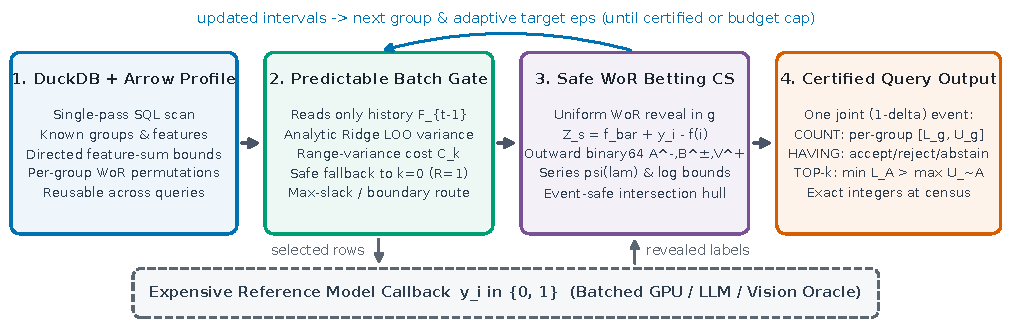
\includegraphics[width=\textwidth]{fig1_architecture.pdf}
\Description{Four-stage architecture diagram of StratQ showing DuckDB and Arrow profiling, the predictable Safe-LOO batch gate, the outward-rounded without-replacement betting confidence sequence, certified query outputs, and the batched expensive reference-model callback loop.}
\caption{\textsc{StratQ} execution architecture. One DuckDB/Arrow profiling stage materializes group indices, directed feature-sum bounds, and per-group permutations that can be reused across multiple queries. During execution, a predictable batch gate reads only revealed history $\mathcal{F}_{t-1}$, routes batched calls to the expensive reference model, and updates outward-rounded binary64 confidence sequences governing \texttt{COUNT}, \texttt{HAVING}, and \texttt{TOP-$k$} outputs.}
\label{fig:arch}
\end{figure*}

\subsection{Columnar Profiling and Arrow Transfer}
\label{sec:sys-profile}

When initialized on a Parquet file or Arrow table, \textsc{StratQ} runs one profiling stage with column pruning: only the grouping key, proxy score column, optional relational covariates, and (for offline replay) label column are projected. The stage first issues a DuckDB aggregate query for group cardinalities and feature extrema, then a column-pruned Arrow query. DuckDB exposes Arrow buffers without an obligatory copy at that boundary; conversion to Python group lists, NumPy arrays, and the stacked feature matrix materializes new arrays.
From these arrays, the profiler builds an in-memory reusable \texttt{TableProfile} containing:
\begin{enumerate}
  \item Contiguous per-group row-index slices $\{I_g\}_{g \in \mathcal{G}}$ constructed in $O(N \log N)$ via a single stable \texttt{argsort} and \texttt{bincount} split;
  \item Normalized feature matrix $\Phi \in [0, 1]^{N \times d}$ (intercept, normalized proxy score, and optional covariates);
  \item Per-group directed feature-sum envelopes $[\Phi_{\text{sum},g}^-, \Phi_{\text{sum},g}^+]$ (computed via the Higham reduction bound of \S\ref{sec:fp64}) and feature-wise extrema $[\phi_{\min,g}, \phi_{\max,g}]$.
\end{enumerate}

Crucially, for any linear predictor $f_s(i) = \theta^\top \phi_i$, the remaining-population mean $\bar{f}_s$ is updated in $O(d)$ time per revealed row by subtracting the running observed feature sum from the directed total sum interval $[\Phi_{\text{sum},g}^-, \Phi_{\text{sum},g}^+]$ and dividing by $m_s = N_g - s + 1$.
For group sizes $N_g \le 25{,}000$, \textsc{StratQ} evaluates exact linear predictor extrema $\min_{i \in I_g} \theta^\top \phi_i$ and $\max_{i \in I_g} \theta^\top \phi_i$ with outward rounding; for larger groups (e.g., 10M-row snapshots), it computes $O(d)$ outward-rounded box bounds from $[\phi_{\min,g}, \phi_{\max,g}]$, keeping per-batch metadata cost independent of $N_g$.
Because the live-callback profile stores no reference labels, its feature/group metadata can be reused across follow-up queries with different reference predicates, tolerances, thresholds $\tau_{\text{cnt}}$, or $k$ values (\S\ref{sec:eval-systems}). Offline replay instead stores the label column in the profile and is reported separately; in both modes the predictor features are specific to the profiled proxy/covariates.

\subsection{Unified Execution Loop and Adaptive Routing}
\label{sec:sys-exec}

Algorithm~\ref{alg:stratq} unifies execution across \texttt{COUNT}, \texttt{HAVING}, and \texttt{TOP-$k$}.
At query start, the engine draws an independent uniform permutation $\pi_g$ per group (never exposed to the predictor or scheduler beyond revealed prefixes) and reveals a small uniform pilot prefix $p_0$ per group, capped by $N_g$ and $B_{\max}$.
Input validation strictly enforces $y_i \in \{0, 1\}$ (rejecting \texttt{NaN} or out-of-domain outputs) and verifies that the reference callback returns exactly one label per requested row ID.

\begin{algorithm}[t]
\small
\caption{\textsc{StratQ} Certified Grouped Query Execution}
\label{alg:stratq}
\KwIn{Profile $\mathcal{P}$, reference callback $\mathcal{O}$, query mode $Q \in \{\texttt{COUNT}, \texttt{HAVING}, \texttt{TOP-}k\}$, risk $\delta$, batch size $b$, pilot $p_0$, budget cap $B_{\max}$}
\KwOut{Certified intervals $\{[L_g, U_g]\}_{g\in\mathcal{G}}$ and query-specific decision}
Initialize per-group risk $\alpha_g \leftarrow \delta/G$, uniform permutation $\pi_g$, and safe CS state $\mathcal{C}_g$ from $\mathcal{P}$\;
Reveal pilot prefix of $\min(p_0, N_g)$ rows per group under the fixed raw-proxy initialization $\theta_{\text{init}}=(0,1,0,\ldots)$ (respecting $B_{\max}$)\;
$t_{\text{total}} \leftarrow \sum_g t_g$\;
\While{$t_{\text{total}} < B_{\max}$ \textbf{and} not \textsc{Certified}$(Q, \{\mathcal{C}_g\})$}{
  Periodically refit pooled ridge $\theta_{\text{global}}$ on all revealed labels $\mathcal{F}_{t-1}$\;
  Select next group(s) $\mathcal{S} \leftarrow \textsc{Route}(Q, \{\mathcal{C}_g\})$ using only $\mathcal{F}_{t-1}$\;
  \lIf{$\mathcal{S} = \emptyset$}{\textbf{break}}
  \ForEach{$g \in \mathcal{S}$}{
    Compute predictable target $\epsilon_{\text{eff}}$ from $Q$ and $\mathcal{C}_g$\;
    $(\theta_g, [f_{\min,g}^-, f_{\max,g}^+]) \leftarrow \textsc{SafeLOOGate}(\mathcal{F}_{t-1}, g, \theta_{\text{global}}, \epsilon_{\text{eff}})$\;
    $k \leftarrow \min(b, N_g - t_g, B_{\max} - t_{\text{total}})$; \lIf{$k = 0$}{\textbf{continue}}
    $\text{rows} \leftarrow \pi_g[t_g : t_g + k]$; \quad $y \leftarrow \mathcal{O}(\text{rows})$\;
    Update $\mathcal{C}_g$ in reveal order with outward binary64 rounding; $t_g \leftarrow t_g + k$; $t_{\text{total}} \leftarrow t_{\text{total}} + k$\;
  }
}
\Return{Count intervals $\{[L_g, U_g]\}$ (exact integers at $t_g=N_g$) and certified decision / abstention for $Q$}\;
\end{algorithm}

\paragraph{Query-specific routing policies}
All three routing rules inspect only revealed interval state $\mathcal{F}_{t-1}$:
\begin{itemize}
  \item \textbf{Grouped \texttt{COUNT} (width-first max-slack).} Score each non-exhausted group by its normalized slack $s_g = \frac{(U_g - L_g)/2}{\max(\epsilon_g, 10^{-12})}$ if $(U_g - L_g)/2 > \epsilon_g$, else $0$. Route the next batch to $g^* = \arg\max_g s_g$.
  \item \textbf{Grouped \texttt{HAVING} (unresolved-boundary width-first).} Identify unresolved groups satisfying $L_g < \tau_{\text{cnt}} \le U_g$; route the next batch to the unresolved group with the largest normalized rate half-width $(U_g - L_g)/(2 N_g)$. Stop once no unresolved groups remain.
  \item \textbf{Grouped \texttt{TOP-$k$} (LUCB-style boundary pair).} Rank groups by interval midpoint (ties broken by stable secondary key) into candidate top-$k$ set $A$ and complement $\mathcal{G} \setminus A$. Let $g_{\text{in}} = \arg\min_{g \in A} L_g$ and $g_{\text{out}} = \arg\max_{h \notin A} U_h$. If $L_{g_{\text{in}}} > U_{g_{\text{out}}}$, certify $A$ and stop. Otherwise, draw from the non-exhausted members of $\{g_{\text{in}}, g_{\text{out}}\}$ (falling back to the widest non-exhausted group if both boundary groups reached census while other intervals still overlap).
\end{itemize}

\paragraph{Scalar directed-rounding engineering}
During profiling of our initial \texttt{safe\_rounding=True} implementation, we observed that dispatching scalar binary64 enclosures through NumPy array checks (\texttt{np.asarray}/\texttt{np.all}) and recomputing the 96-term $\psi(\lambda)$ series inside Python loops caused 2,280 reveal steps to take 7.69\,s (and 32,512 steps at 10M rows to take 276.5\,s).
Replacing the inner scalar enclosures with native Python \texttt{float}/\texttt{math.nextafter} fast paths and LRU-caching \texttt{psi\_e\_enclosure} (preserving bit-for-bit identical outward bounds and verified against the 50-digit \texttt{Decimal} suite) reduced the same 2,280-step benchmark from 7,689.2\,ms to 209.9\,ms ($36.6\times$ speedup) and reduced 10M-row warm query time to 2.83\,s (\S\ref{sec:eval-systems}).
This makes the statistical engine overhead negligible relative to GPU neural or LLM reference inference.

\section{Evaluation}
\label{sec:eval}

We evaluate \textsc{StratQ} across six workload families and eleven database/modern operator adaptations plus an independent grouped hypergeometric CS to answer five questions:
(Q1) Does \textsc{StratQ} achieve real end-to-end latency speedups and reliable decision certification on expensive GPU neural predicates?
(Q2) How does \textsc{StratQ} compare against modern 2025--2026 statistical and database comparators (\texttt{Spertus-WoR}, \texttt{CELEUS-FixedProxy}, \texttt{Calibrated-FixedProxy}, \texttt{BARGAIN-Global}, \texttt{PilotDB-Asymp})?
(Q3) Does Safe-LOO range--variance gating deliver strong savings on accurate proxies without degrading under noisy or weak proxies?
(Q4) How do \textsc{StratQ}'s guarantees and cost behave across classical grouped AQP baselines, decision boundaries, and high group counts under Zipf skew?
(Q5) How do DuckDB+Arrow profiling, query reuse, and isolated memory footprint scale to 10 million rows?

\subsection{Experimental Setup and Comparators}
\label{sec:eval-setup}

\paragraph{Environment}
All experiments run on Windows 11 with Python 3.12, DuckDB 2.0.1, PyArrow 21.0, PyTorch 2.8.0 (CUDA 12.9), and an NVIDIA GeForce RTX 4060 Laptop GPU (8\,GiB VRAM).
Unless noted otherwise, every \textsc{StratQ} arm enforces nominal $90\%$ joint simultaneous coverage ($\delta = 0.1$) with \texttt{gating\_mode="safe\_loo"} and \texttt{safe\_rounding=True}; external adaptations use their documented interval implementations.

\paragraph{Six workload families}
(1)~\textbf{Yelp-DistilBERT-SST2} (live GPU text): 20,000 Yelp test reviews partitioned into $G=5$ star-rating groups ($N_g \in [3{,}791, 4{,}108]$); reference predicate is DistilBERT-SST2 on GPU (batch 64/128/256), and proxy is a CPU TF-IDF + Logistic Regression trained on a disjoint 18,000-row prefix.
(2)~\textbf{CIFAR10-ResNet34-GPU} (live GPU vision): 10,000 CIFAR-10 test images across $G=10$ classes ($N_g = 1{,}000$ each); reference predicate is an ImageNet-pretrained ResNet34 fine-tuned and evaluated on GPU at standard $224\times 224$ resolution to detect animal classes, and proxy is a CPU logistic model on $4\times 4$ RGB averages plus channel standard deviations (51 features).
(3)~\textbf{Fashion-MNIST} (live CPU vision): 10,000 official test images in $G=5$ brightness bins; RBF-SVM reference vs.\ pooled-pixel logistic proxy ($\epsilon_g = 0.04 N_g$).
(4)~\textbf{SMS Spam} (live CPU text): 2,271 deduplicated held-out messages across $G=5$ length groups; character-feature $k$-NN reference vs.\ word-feature logistic proxy ($\epsilon_g = 0.06 N_g$).
(5)~\textbf{UCI Adult} (tabular replay): 16,281 official test rows across $G=9$ workclass groups ($\epsilon_g = 0.04 N_g$), using education-rate proxy plus \texttt{age} and \texttt{hours} covariates.
(6)~\textbf{Synthetic Parquet Scale \& Stress}: 12K-row proxy-quality sweep ($G=8$), 100K-row Zipf skew sweep ($G \in \{5,10,20,50,100\}$, $\alpha_{\text{zipf}} \in \{0.0, 0.8, 1.2\}$), and 100K--10M-row Parquet snapshots ($G=20$).

\paragraph{Eleven operator comparators}
We separate \emph{modern 2025--2026 operator adaptations} from \emph{classical AQP operators}; none is claimed as a full system replica, and all contract differences are audited in our artifact documentation.
Modern comparators:
\textbf{Spertus-WoR} (adapted from~\cite{spertus2026sequential}: uniform within-group WoR, max-slack routing, zero predictor, Bonferroni risk);
\textbf{CELEUS-FixedProxy} (adapted from~\cite{zhou2026celeus}: fixed surrogate-completed IPW signal and hedged-capital e-process inversion across groups);
\textbf{Calibrated-FixedProxy} (independent control, not a named system replica: one Ridge predictor fitted on the same pilot prefix and frozen permanently while sharing \textsc{StratQ}'s permutations, routing, and safe CS);
\textbf{BARGAIN-Global} (adapted from~\cite{zeighami2026bargain}: single global anytime count target with proportional plug-in group estimates); and
\textbf{PilotDB-Asymp} (adapted from~\cite{zhu2025pilotdb}: two-stage CLT simultaneous normal intervals with finite-population correction, evaluated under an optional-stopping diagnostic to expose asymptotic failure).
Classical comparators on Adult (at matched budgets $B \in \{2{,}048, 4{,}096, 8{,}192\}$): \textbf{ABae-inspired} two-stage proxy strata~\cite{kang2021abae}, \textbf{BlazeIt-inspired} fixed-look control-variate EB~\cite{kang2019blazeit}, \textbf{Congressional Senate} equal-quota hypergeometric~\cite{acharya2000congress}, \textbf{Online Aggregation} unindexed Hoeffding scan~\cite{hellerstein1997online}, \textbf{LWS} Des Raj normal~\cite{walenz2019lws}, and \textbf{VerdictDB} variational subsampling~\cite{park2018verdict}. An independent grouped hypergeometric CS~\cite{wor2020} is reported separately, yielding twelve non-\textsc{StratQ} methods in total.

\subsection{Live GPU Workloads and Modern Comparators}
\label{sec:eval-gpu}

\begin{figure*}[t]
\centering
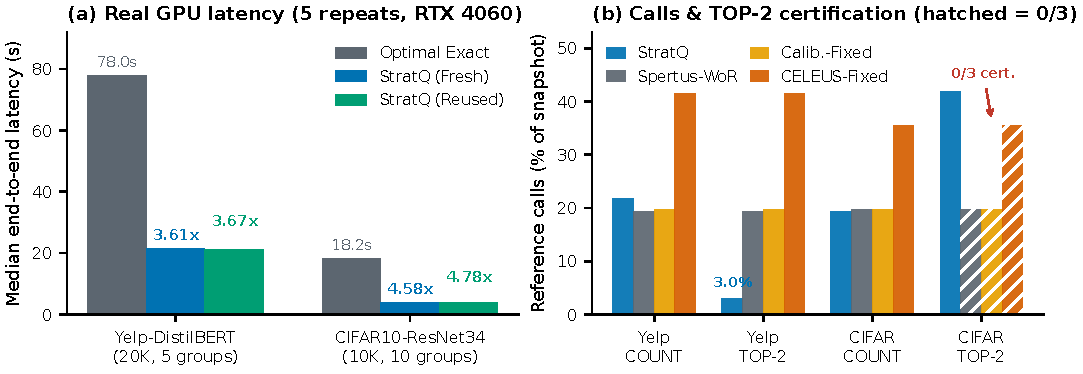
\includegraphics[width=\textwidth]{fig2_gpu_workloads.pdf}
\Description{Two-panel figure comparing StratQ against optimal exact GPU inference and modern operator baselines on Yelp-DistilBERT-SST2 and CIFAR10-ResNet34-224 after proxy scoring, showing 3.61x to 4.78x ratio-of-medians speedups and certified TOP-2 call efficiency under dedicated versus post-hoc COUNT-derived routing.}
\caption{Live GPU evaluation on RTX 4060 after proxy scoring. (a) Median grouped \texttt{COUNT} latency over 5 repeats vs.\ the fastest tested exact GPU batch size (batch 128 on Yelp, 64 on CIFAR-10); fresh/reused profiles win at modeled $Q=1$ under this setup boundary. (b) Reference calls (\% of snapshot) for \texttt{COUNT} and \texttt{TOP-2}; hatched bars indicate $0/3$ certification on CIFAR-10's 2-image rank gap under the post-hoc \texttt{COUNT}-derived protocol.}
\label{fig:gpu}
\end{figure*}

\begin{table*}[t]
\centering
\footnotesize
\setlength{\tabcolsep}{4pt}
\caption{Live GPU expensive-predicate evaluation (3 seeds per query, $\delta=0.1$, $\epsilon_g=0.04 N_g$). Calls are means; sample SD and ranges are reported in the text. \texttt{COUNT Wall} excludes profile construction. \texttt{BARGAIN-Global} satisfies only a global target ($0/3$ all-group coverage). For non-\textsc{StratQ} baselines, \texttt{HAVING}/\texttt{TOP-2} decisions are derived from their \texttt{COUNT} intervals; \textsc{StratQ} runs dedicated boundary-focused routing under the same joint event.}
\label{tab:gpu-main}
\begin{tabular}{@{}llrrrrrr@{}}
\toprule
Workload & Method & \texttt{COUNT} Calls (\%) & Cov. & \texttt{COUNT} Wall (s) & \texttt{HAVING} Calls (Res./Corr.) & \texttt{TOP-2} Calls (Cert./Corr.) & Speedup vs.\ Exact \\
\midrule
\multirow{5}{*}{\shortstack[l]{Yelp-DistilBERT\\(20K, $G=5$,\\Exact 77.99\,s)}}
& \textbf{\textsc{StratQ} (\texttt{safe\_loo})} & 4,349 (21.7\%) & \textbf{3/3} & 17.47 & 4,390 (\textbf{3/3} / \textbf{3/3}) & \textbf{595 (3.0\%)} (\textbf{3/3} / \textbf{3/3}) & \textbf{3.61$\times$ / 3.67$\times$} \\
& Spertus-WoR~\cite{spertus2026sequential} & \textbf{3,859} (19.3\%) & 3/3 & 15.95 & 3,859 (0/3 / 3/3) & 3,859 (19.3\%) (3/3 / 3/3) & --- \\
& Calibrated-FixedProxy & 3,944 (19.7\%) & 3/3 & 15.43 & 3,944 (0/3 / 3/3) & 3,944 (19.7\%) (3/3 / 3/3) & --- \\
& CELEUS-FixedProxy~\cite{zhou2026celeus} & 8,296 (41.5\%) & 3/3 & 33.56 & 8,296 (0/3 / 3/3) & 8,296 (41.5\%) (3/3 / 3/3) & --- \\
& BARGAIN-Global~\cite{zeighami2026bargain} & 819 (4.1\%) & \textbf{0/3} & 3.13 & 819 (0/3 / \textbf{0/3}) & 819 (4.1\%) (0/3 / \textbf{0/3}) & --- \\
\midrule
\multirow{5}{*}{\shortstack[l]{CIFAR10-ResNet34\\(10K, $G=10$,\\Exact 18.22\,s)}}
& \textbf{\textsc{StratQ} (\texttt{safe\_loo})} & \textbf{1,936 (19.4\%)} & \textbf{3/3} & \textbf{2.82} & 4,421 (\textbf{3/3} / \textbf{3/3}) & \textbf{4,187 (41.9\%)} (\textbf{3/3} / \textbf{3/3}) & \textbf{4.58$\times$ / 4.78$\times$} \\
& Spertus-WoR~\cite{spertus2026sequential} & 1,979 (19.8\%) & 3/3 & 2.85 & 1,979 (0/3 / 3/3) & 1,979 (19.8\%) (\textbf{0/3} / \textbf{0/3}) & --- \\
& Calibrated-FixedProxy & 1,979 (19.8\%) & 3/3 & 2.97 & 1,979 (0/3 / 3/3) & 1,979 (19.8\%) (\textbf{0/3} / \textbf{0/3}) & --- \\
& CELEUS-FixedProxy~\cite{zhou2026celeus} & 3,557 (35.6\%) & 3/3 & 5.07 & 3,557 (0/3 / 3/3) & 3,557 (35.6\%) (\textbf{0/3} / 1/3) & --- \\
& BARGAIN-Global~\cite{zeighami2026bargain} & 733 (7.3\%) & \textbf{0/3} & 1.13 & 733 (3/3 / \textbf{0/3}) & 733 (7.3\%) (\textbf{0/3} / \textbf{0/3}) & --- \\
\bottomrule
\end{tabular}
\end{table*}

Figure~\ref{fig:gpu} and Table~\ref{tab:gpu-main} summarize both live GPU workloads (peak VRAM 1.29\,GiB on Yelp and 2.03\,GiB on CIFAR-10).

\paragraph{Descriptive variability (three seeds).}
\texttt{COUNT} calls are mean $\pm$ sample SD [range]: on Yelp, \textsc{StratQ} $4{,}349\pm74$ [4{,}264, 4{,}392] vs.\ Spertus-WoR $3{,}859\pm98$ [3{,}752, 3{,}944]; on CIFAR-10, $1{,}936\pm128$ [1{,}808, 2{,}064] vs.\ $1{,}979\pm133$ [1{,}872, 2{,}128]. Decision-call SD/ranges are in the artifact. These fixed-snapshot results are descriptive, not significance tests or population coverage estimates.

\paragraph{Query-level GPU latency after proxy scoring.}
Five repeats (seeds 5000--5004; tolerances 3/4/5/3/4\%) give median [range] latency: Yelp 77.99 [65.46, 87.78]\,s exact, 21.62 [14.22, 27.32]\,s fresh-profile, and 21.24 [14.73, 28.19]\,s reused; CIFAR-10 18.22 [17.74, 18.58]\,s, 3.98 [3.37, 5.30]\,s, and 3.81 [3.42, 5.23]\,s. Ratio-of-medians speedups are \textbf{3.61$\times$ fresh / 3.67$\times$ reused} and \textbf{4.58$\times$ / 4.78$\times$}. Proxy scores are precomputed and the GPU model/OS cache is warm; ``fresh'' only rebuilds the \texttt{TableProfile}, and the frozen run shared the $\psi$ cache. Fitting, loading, and proxy scanning are excluded. Adding Yelp's 3.97\,s scan gives 3.05$\times$/3.09$\times$; adding 6.75\,s training as first-query setup gives 2.41$\times$ fresh. CIFAR's scan time was not recorded.

\paragraph{Decision certification vs.\ modern comparators}
The sharpest separation emerges on SQL decision queries:
\begin{itemize}
  \item \textbf{Yelp \texttt{TOP-2} and \texttt{HAVING}:} Groups 4 and 5 (3,398 and 3,406 positives) separate from group 3 (2,178). With dedicated boundary routing, \textsc{StratQ} certifies exact \texttt{TOP-2} membership in \textbf{594.7 reference calls ($3.0\%$ of rows)} with $3/3$ accuracy---$6.5\times$ fewer than the Spertus-WoR adaptation (3,858.7), $6.6\times$ fewer than Calibrated-FixedProxy (3,944.0), and $13.9\times$ fewer than CELEUS-FixedProxy (8,296.0). On \texttt{HAVING} ($\tau=2{,}178$, exactly group 3's true count), it resolves all groups $3/3$ correctly, whereas the post-hoc \texttt{COUNT}-derived protocol leaves the boundary group unresolved ($0/3$ fully resolved). The global-count surrogate misclassifies groups ($0/3$ correct); this does not evaluate BARGAIN's original global guarantee.
  \item \textbf{CIFAR-10 \texttt{COUNT} and extreme 2-image \texttt{TOP-2}:} On \texttt{COUNT}, \textsc{StratQ} uses 1,936.0 calls (2.82\,s), vs.\ 1,978.7 for Spertus-WoR and Calibrated-FixedProxy and 3,557.3 for CELEUS-FixedProxy. On \texttt{HAVING} ($\tau=979$), dedicated routing resolves all groups $3/3$, while the post-hoc protocol fully resolves $0/3$. On \texttt{TOP-2}, the top four animal classes have true counts $(999, 996, 994, 993)$---only \textbf{2 images} between ranks 2 and 3. \textsc{StratQ} certifies the exact set in $3/3$ runs (4,186.7 calls, $41.9\%$ of rows). Under their respective \texttt{COUNT} stopping budgets, the post-hoc comparators certify $0/3$ and return wrong point rankings ($0/3$ or $1/3$); this does not establish how equal-budget decision-aware baseline routing would perform.
\end{itemize}

\paragraph{Honest boundary observation on Yelp \texttt{COUNT}.}
\textsc{StratQ} uses $4{,}349\pm74$ calls vs.\ $3{,}859\pm98$ for Spertus-WoR and $3{,}944\pm64$ for Calibrated-FixedProxy (mean$\pm$SD, $n=3$). A 202-decision trace selects a proxy in 112 batches, falls back for no cost improvement in 75, and for insufficient history in 15. Selected candidates reduce mean LOO variance by 12.9\%, but maximum prediction span is $8.9\times10^{-16}$ and none has $R>1.01$; the range-penalty explanation is therefore unsupported. Group-label variances are 0.067--0.249, not uniformly tiny. The defensible conclusion is that the LOO surrogate does not guarantee realized call dominance. \textsc{StratQ} remains $1.91\times$ cheaper than CELEUS-FixedProxy (8,296.0).

\subsection{Proxy Quality Sweep, Safe-LOO Ablation, and Zipf Stress}
\label{sec:eval-systems}

\begin{figure*}[t]
\centering
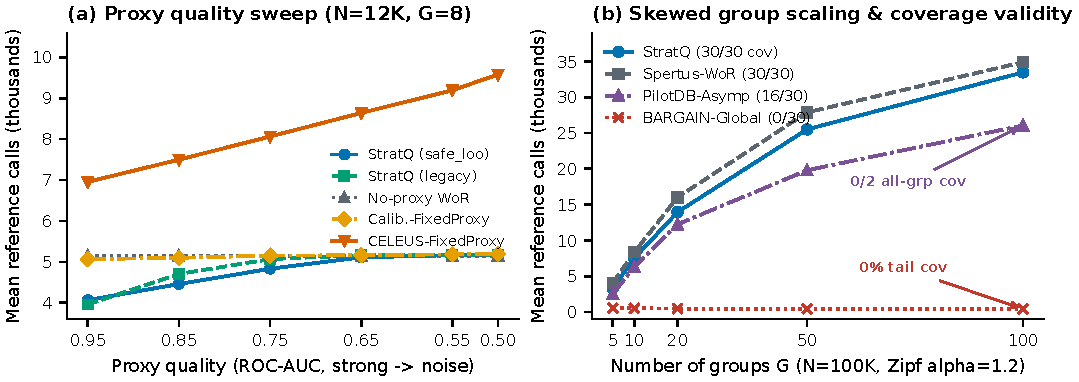
\includegraphics[width=\textwidth]{fig3_proxy_sweep_zipf.pdf}
\Description{Two-panel plot showing (a) reference calls across proxy ROC-AUC from 0.95 down to 0.50 where Safe-LOO achieves strong savings at high AUC and near-zero degradation at noise, and (b) Zipf group scaling from G=5 to G=100 showing StratQ 30/30 coverage vs PilotDB 16/30 and BARGAIN 0/30.}
\caption{(a) Proxy quality sweep ($N=12\text{K}$, $G=8$, 3 seeds): \texttt{safe\_loo} saves up to $21.1\%$ calls at AUC $0.95$, leads all comparators at moderate AUC ($0.75$--$0.85$), and stays within $+0.21\%$ of no-proxy WoR under pure noise (AUC $0.50$), whereas \texttt{CELEUS-FixedProxy} degrades to $9{,}579$ calls. (b) Skewed group scaling ($N=100\text{K}$, $\alpha=1.2$): across all 15 $(G,\alpha)$ configurations (two seeds each), \textsc{StratQ} covers all groups in $30/30$ runs, the optional-stopping CLT diagnostic in $16/30$, and the global-count surrogate's proportional group intervals in $0/30$. Coverage labels aggregate all $\alpha$ values.}
\label{fig:sweep-zipf}
\end{figure*}

\paragraph{Proxy quality sweep (AUC $0.95 \to 0.50$)}
Figure~\ref{fig:sweep-zipf}(a) isolates proxy quality on a fixed 12,000-row, 8-group Zipf snapshot ($\epsilon_g = 0.04 N_g$, 3 seeds).
At strong proxy quality (AUC $0.95$), \texttt{safe\_loo} reduces mean calls from 5,152 (\texttt{no\_proxy}) to \textbf{4,064} ($-21.1\%$), outperforming \texttt{Calibrated-FixedProxy} (5,067) and \texttt{CELEUS-FixedProxy} (6,955). The corresponding sample SDs are $32$ vs.\ $85$ calls; at AUC $0.50$, \texttt{safe\_loo} is $5{,}163\pm121$ vs.\ $5{,}152\pm85$ for no-proxy.
At moderate quality (AUC $0.85$ and $0.75$), \texttt{safe\_loo} is the single best method (4,459 and 4,832 calls), beating both \texttt{legacy} (4,704 and 5,067) and \texttt{Calibrated-FixedProxy} (5,099 and 5,152).
As the proxy degrades to near-noise and pure noise (AUC $0.55$ and $0.50$), \texttt{safe\_loo}'s LOO guard triggers fallback to $\kappa=0$, holding calls at \textbf{5,163} ($+0.21\%$ vs.\ 5,152, $3/3$ coverage).
In contrast, \texttt{CELEUS-FixedProxy} climbs monotonically to \textbf{9,579 calls} ($+85.9\%$ overhead) with $2/3$ coverage at AUC $\le 0.65$.

\paragraph{Safe-LOO ablation on Adult, SMS, and Fashion-MNIST}
Figure~\ref{fig:s1-adult}(a) and Table~\ref{tab:s1-ablation} report our matched 195-run Sprint~1 ablation (\texttt{legacy} vs.\ \texttt{safe\_loo} vs.\ \texttt{no\_proxy}, all with \texttt{safe\_rounding=True}).
On strong-proxy \textbf{Fashion-MNIST}, \texttt{safe\_loo} cuts mean calls by \textbf{$61.26\%$} (from 3,510.4 to \textbf{1,360.0}, improving even over \texttt{legacy}'s 1,411.2) while achieving the narrowest mean half-width ($3.36\%$).
On \textbf{SMS}, \texttt{safe\_loo} reduces \texttt{COUNT} calls by \textbf{$14.01\%$} (816.8 $\to$ 702.4) and remains below no-proxy on both decision queries (\texttt{HAVING}: $-1.67\%$, 863.1 $\to$ 848.7; \texttt{TOP-2}: $-0.90\%$, 865.9 $\to$ 858.1), with $10/10$ correct decisions and $10/10$ \texttt{TOP-2} certifications. It does \emph{not} beat the legacy selector: legacy uses 689.6, 835.9, and 853.2 calls on these three queries, respectively. All modes cover all groups in every run.
On weak-proxy \textbf{Adult} (with \texttt{age} and \texttt{hours} covariates), \texttt{safe\_loo} uses 4,378.0 calls vs.\ 4,337.5 for \texttt{no\_proxy} ($+0.93\%$, $30/30$ coverage), confirming that weak proxies can still incur a sub-$1\%$ gating overhead when betting steps approach the $\lambda \le 0.5$ cap.
All $195/195$ runs covered every group's true count.

\begin{figure*}[t]
\centering
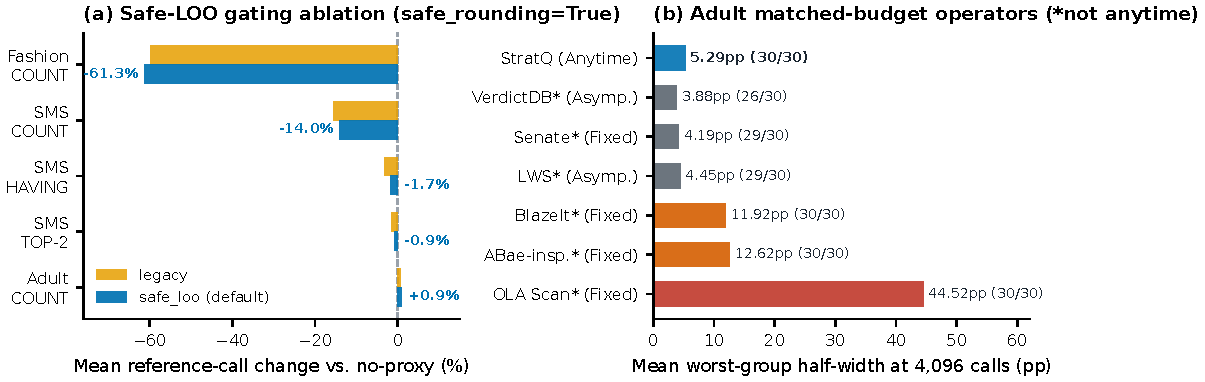
\includegraphics[width=\textwidth]{fig4_sprint1_adult.pdf}
\Description{Two-panel figure showing (a) Sprint 1 Safe-LOO vs legacy call reduction on Fashion-MNIST, SMS, and Adult, and (b) Adult 4,096-call matched-budget worst-group half-widths and simultaneous coverage across StratQ and six classical database operators.}
\caption{(a) Matched 195-run ablation (\texttt{safe\_rounding=True}): \texttt{safe\_loo} saves $61.3\%$ calls on Fashion-MNIST and $14.0\%$ on SMS \texttt{COUNT}, remains below no-proxy on SMS decisions but does not beat legacy, and limits weak-proxy Adult overhead to $+0.9\%$. (b) Adult matched-budget ($B=4{,}096$) worst-group half-width and joint coverage ($30$ seeds). Among these six fixed-look/asymptotic adaptations, only \textsc{StratQ} uses a finite-sample anytime stopping rule; the independent hypergeometric CS in the text is also anytime.}
\label{fig:s1-adult}
\end{figure*}

\begin{table}[t]
\centering
\footnotesize
\setlength{\tabcolsep}{3.5pt}
\caption{Matched 195-run Safe-LOO ablation (\texttt{safe\_rounding=True}, $\delta=0.1$). ``Max HW'' is the mean over runs of each run's largest per-group half-width. All trials achieved 100\% joint group coverage and target/decision correctness.}
\label{tab:s1-ablation}
\begin{tabular}{@{}llrrr@{}}
\toprule
Workload & Mode & Mean Calls & $\Delta$ vs.\ No-Proxy & Max HW \\
\midrule
\multirow{3}{*}{Fashion COUNT (5)}
& \texttt{no\_proxy} & 3,510.4 & 0.0\% & 3.96\% \\
& \texttt{legacy} & 1,411.2 & $-59.80\%$ & 3.84\% \\
& \textbf{\texttt{safe\_loo}} & \textbf{1,360.0} & \textbf{$-61.26\%$} & \textbf{3.59\%} \\
\midrule
\multirow{3}{*}{SMS COUNT (10)}
& \texttt{no\_proxy} & 816.8 & 0.0\% & 5.88\% \\
& \texttt{legacy} & 689.6 & $-15.57\%$ & 5.71\% \\
& \textbf{\texttt{safe\_loo}} & \textbf{702.4} & \textbf{$-14.01\%$} & \textbf{5.67\%} \\
\midrule
\multirow{3}{*}{SMS HAVING (10)}
& \texttt{no\_proxy} & 863.1 & 0.0\% & 28.11\% \\
& \texttt{legacy} & 835.9 & $-3.15\%$ & 27.43\% \\
& \textbf{\texttt{safe\_loo}} & \textbf{848.7} & \textbf{$-1.67\%$} & 29.71\% \\
\midrule
\multirow{3}{*}{SMS TOP-2 (10)}
& \texttt{no\_proxy} & 865.9 & 0.0\% & 29.18\% \\
& \texttt{legacy} & 853.2 & $-1.47\%$ & 27.43\% \\
& \textbf{\texttt{safe\_loo}} & \textbf{858.1} & \textbf{$-0.90\%$} & 29.71\% \\
\midrule
\multirow{3}{*}{Adult COUNT (30)}
& \texttt{no\_proxy} & 4,337.5 & 0.0\% & 3.97\% \\
& \texttt{legacy} & 4,369.5 & $+0.74\%$ & 3.97\% \\
& \texttt{safe\_loo} & 4,378.0 & $+0.93\%$ & 3.97\% \\
\bottomrule
\end{tabular}
\end{table}

\paragraph{High group counts and Zipf skew stress}
Figure~\ref{fig:sweep-zipf}(b) reports our 100K-row Zipf stress suite spanning $G \in \{5, 10, 20, 50, 100\}$ and $\alpha_{\text{zipf}} \in \{0.0, 0.8, 1.2\}$ (AUC $0.85$, $\epsilon_g = 0.05 N_g$, 2 seeds per cell = 30 runs per method).
\textsc{StratQ} achieves \textbf{$30/30$ ($100\%$) all-group coverage} and $100\%$ tail-group coverage across every cell, while using fewer calls than \texttt{Spertus-WoR} in \textbf{14 of 15} $(G, \alpha)$ configurations (e.g., at $G=100, \alpha=0.0$: 62,784 vs.\ 71,424 calls, saving 8,640 calls; at $G=20, \alpha=1.2$: 13,952 vs.\ 16,000; only at $G=5, \alpha=0.0$ is \textsc{StratQ} slightly higher at 3,856 vs.\ 3,664).
The global-count surrogate's proportional group intervals cover all groups in \textbf{$0/30$} runs and $0/222$ tail-group instances; the JSON does not record its global interval, so this is not a test of BARGAIN's original guarantee. The \texttt{PilotDB-Asymp} optional-stopping diagnostic covers all groups in \textbf{$16/30$ ($53.3\%$)} runs and $0/6$ at $G=100$, with pooled tail coverage $215/222=96.85\%$. Reusing a fixed-look CLT radius at data-dependent looks is a diagnostic protocol mismatch, not PilotDB's intended fixed-look use.
Optimizer overhead for \textsc{StratQ} scales cleanly from 0.32\,s ($G=5$) to 3.01\,s ($G=100, \alpha=1.2$, 33.5K calls).

\subsection{Classical Baselines, Decision Boundaries, and Routing}
\label{sec:eval-classical}

\paragraph{Six classical AQP operators on Adult}
Figure~\ref{fig:s1-adult}(b) compares \textsc{StratQ} against six published sampling/interval operators at a matched budget of $B=4{,}096$ calls on UCI Adult (30 seeds).
Only \textsc{StratQ} maintains finite-sample anytime validity across all stopping times; at 4,096 calls its mean worst-group half-width is \textbf{5.29\,pp} ($30/30$ coverage), outperforming fixed-look \textbf{BlazeIt-inspired} (11.92\,pp, $30/30$), \textbf{ABae-inspired} proxy strata (12.62\,pp, $30/30$), and unindexed \textbf{Online Aggregation} (44.52\,pp, $30/30$, where $15/30$ runs leave at least one small group completely unsampled).
Fixed-look \textbf{Senate} (4.19\,pp, $29/30$), asymptotic \textbf{LWS} (4.45\,pp, $29/30$), and asymptotic \textbf{VerdictDB} (3.88\,pp, observed $26/30$) produce narrower single-look intervals at $B=4{,}096$, illustrating the modest width price paid for finite-sample optional-stopping validity. The $26/30$ observation is not itself proof of sub-nominal population coverage.
An independent anytime grouped hypergeometric CS~\cite{wor2020} requires $4{,}581.7\pm178.8$ mean$\pm$SD calls on Adult vs.\ $4{,}337.5\pm84.8$ for no-proxy \textsc{StratQ} ($30/30$ coverage each), a 244.3-call (5.63\%) gap.

\paragraph{Decision boundaries and abstention (960 runs)}
We evaluated four 1,024-row snapshots ($G=4$, $N_g=256$) with counts $(192,128,128-d,32)$, $d\in\{0,1,16,64\}$, three budgets $\{256,768,1{,}024\}$, 20 seeds, proxy on/off, and two queries ($4\times3\times20\times2\times2=960$ trials). \textbf{All 960 runs had zero interval-coverage failures, wrong \texttt{HAVING} labels, and wrong certificates;} all 288 certified top-2 runs were correct.
At budget 256 no \texttt{HAVING} run ($\tau=128$) fully resolved. At 768 all positive-gap top-2 runs certified ($120/120$); ties abstained until census ($B=1{,}024$), where deterministic tie-breaking certified $40/40$ runs (20 seeds $\times$ two proxy settings).

\paragraph{Capped-budget routing ablation (180 matched pairs)}
Without a binding budget cap and with the proxy disabled, width-first and round-robin routing consume identical prefixes (4,337.5 mean calls across all 30 Adult seeds).
Under caps $B \in \{2{,}048, 4{,}096, 8{,}192\}$, width-first routing produces a strictly smaller worst-group half-width in \textbf{180/180 matched pairs} (e.g., at $B=4{,}096$ with proxy, mean max half-width drops from 6.67\,pp to 5.29\,pp), while the mean number of groups below 4\% falls from 5.73 to 2.40 out of nine---a direct minimax vs.\ throughput trade-off.

\paragraph{Cheap CPU live latency.}
An aligned rerun (one warm-up + ten randomized measured blocks; identical models/rows and exact batch sweep) gives Fashion-MNIST 1,430.5\,ms exact (best batch 1,024), vs.\ 577.3\,ms fresh and 423.5\,ms reused. SMS is 519.2\,ms exact (full batch), vs.\ 902.3\,ms fresh and 834.7\,ms reused, so exact batching wins. Fitting/loading are excluded. This record supersedes the older cross-study CPU timing comparison.

\subsection{Scale, Profile Amortization, and Memory Attribution}
\label{sec:eval-scale}

\begin{figure*}[t]
\centering
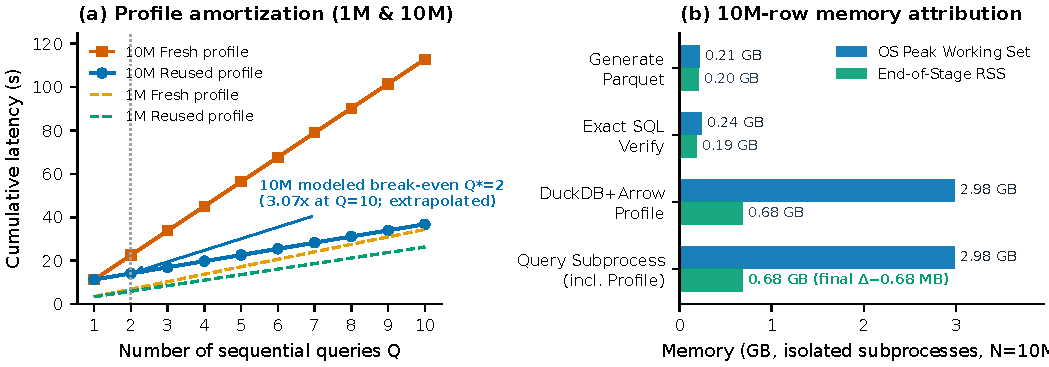
\includegraphics[width=\textwidth]{fig5_scale_memory.pdf}
\Description{Two-panel figure showing (a) cumulative latency of fresh vs reused DuckDB and Arrow profiles at 1M and 10M rows with modeled break-even at Q*=2, and (b) isolated four-stage subprocess memory breakdown at 10M rows showing profile-dominated peak working set, an 85.6 MB query traced-allocation peak, a single +21.7 MB immediate post-query RSS delta, and a -0.68 MB final post-teardown delta.}
\caption{(a) Profile amortization over sequential queries on 1M and 10M Parquet snapshots: at 10M rows, profile reuse breaks even at modeled $Q^*=2$ and achieves $3.07\times$ lower modeled cumulative latency by $Q=10$; only five queries were measured, so $Q=10$ is extrapolated. (b) Independent subprocess memory attribution at $N=10\text{M}$: DuckDB/Arrow profiling accounts for the peak working set (2.98\,GB under \texttt{tracemalloc}; 0.68\,GB end RSS). The query subprocess also rebuilds the profile, so its peak WS is not query-only. A single immediate post-query RSS delta is $+21.7$\,MB, the query-stage traced-allocation peak is 85.6\,MB, and the final post-teardown RSS delta is $-0.68$\,MB.}
\label{fig:scale-mem}
\end{figure*}

\begin{table}[t]
\centering
\footnotesize
\setlength{\tabcolsep}{3.2pt}
\caption{Isolated four-stage subprocess memory attribution at $N=10\text{M}$ rows ($G=20$, offline Boolean-label replay). ``Wall'' is subprocess-stage wall; the query stage rebuilds the profile before its 37.86\,s query-only execution. RSS deltas use the profile-end baseline and are single observations.}
\label{tab:mem-10m}
\begin{tabular}{@{}lrrrr@{}}
\toprule
Stage (Subprocess) & Wall & \texttt{tracemalloc} & Peak WS & End RSS \\
\midrule
Generate Parquet & 1.64\,s & 11.4\,MB & 0.213\,GB & 0.203\,GB \\
Exact SQL Verify & 0.06\,s & 0.0\,MB & 0.236\,GB & 0.186\,GB \\
DuckDB+Arrow Profile & 104.53\,s & 1,285.3\,MB & 2.979\,GB & 0.682\,GB \\
Query Subprocess (incl.\ Prof.) & 187.85\,s & 85.6\,MB & 2.980\,GB & 0.680\,GB \\
\quad Profile Rebuild & 103.50\,s & --- & --- & --- \\
\quad Query-only Execution & 37.86\,s & --- & --- & --- \\
\quad Immediate Post-query $\Delta$RSS & --- & --- & --- & \textbf{$+$21.69\,MB} \\
\quad Final $\Delta$RSS after Teardown & --- & --- & --- & \textbf{$-$0.68\,MB} \\
\bottomrule
\end{tabular}
\end{table}

Figure~\ref{fig:scale-mem} and Table~\ref{tab:mem-10m} evaluate $1\text{M}$ and $10\text{M}$ Parquet rows ($G=20$, offline Boolean-label replay). Without \texttt{tracemalloc}, profiling takes 0.82--0.85\,s at 1M (warm query 2.55--2.58\,s; modeled $Q^*=1$) and 8.47\,s at 10M (cold 11.28\,s, warm 2.83\,s; modeled $Q^*=2$). The 3.07$\times$ speedup at $Q=10$ extrapolates per-query medians beyond the five measured queries.
Each 10M stage ran in a separate subprocess. The query subprocess rebuilds the profile: 187.85\,s total = 103.50\,s profile + 37.86\,s query. Profiling dominates peak WS (2.979\,GB; 0.682\,GB end RSS). The query stage has an 85.6\,MB traced-allocation peak; its immediate post-query RSS delta is $+21.69$\,MB, but the final post-teardown delta is $-0.68$\,MB. These single allocator-sensitive observations are not retained-memory guarantees.

\section{Related Work and Limitations}
\label{sec:related}

Prior research optimizes fixed-budget grouped error, expensive predicate execution, online stopping, model ranking, or single-population prediction-assisted inference.
\textsc{StratQ} brings these threads into a unified fixed-snapshot SQL grouping contract where every group shares a single anytime-valid coverage event that directly certifies \texttt{COUNT}, \texttt{HAVING}, and \texttt{TOP-$k$} outputs or abstains.

\subsection{Grouped Approximate Query Processing}
Grouped AQP has a rich database lineage. Congressional Sampling~\cite{acharya2000congress} allocates offline stratified samples via Senate/House designs; Sample+Seek~\cite{sample2016}, Quickr~\cite{kandula2016quickr}, and ShadowAQP~\cite{shadow2023} add distribution precision, inline/universe sampling, and attribute-oriented allocation/generation. BlinkDB~\cite{agarwal2013blinkdb}, AQP++~\cite{peng2018aqpplus}, VerdictDB~\cite{park2018verdict}, LWS~\cite{walenz2019lws}, ApproxHadoop~\cite{goiri2015approxhadoop}, and ApproxIoT~\cite{wen2018approxiot} cover multi-resolution samples, aggregate cubes, variational subsampling, learned sampling, and MapReduce/edge analytics.
PilotDB~\cite{zhu2025pilotdb} formalizes a-priori simultaneous relative error across groups. These systems target fixed-budget or two-stage CLT bounds. PilotDB excludes aggregates used as \texttt{GROUP BY} keys (e.g., \texttt{GROUP BY COUNT(*)}), not ordinary \texttt{COUNT} outputs. \textsc{StratQ} instead governs every look, route, and budget cap with one finite-sample anytime event.

\subsection{Expensive Predicates and Semantic Engines}
Expensive predicates are an active VLDB/SIGMOD frontier. NoScope~\cite{kang2017noscope}, Probabilistic Predicates~\cite{lu2018pp}, CORE~\cite{yang2022core}, and TASTI~\cite{kang2022tasti} reduce inference through filters, proxies, and semantic indexes without certifying population totals. SUPG~\cite{kang2020supg} provides asymptotic selection precision/recall; BlazeIt~\cite{kang2019blazeit} uses neural control variates with always-valid empirical-Bernstein stopping; InQuest~\cite{russo2023inquest} gives expected $O(1/B)$ error under stationary streams.
LOTUS~\cite{patel2025lotus} provides gold-relative semantic accuracy with fixed-sample CLT/multiplicity corrections; UQE~\cite{dai2024uqe} discovers semantic groups; Palimpzest~\cite{liu2025palimpzest} and DocETL~\cite{shankar2025docetl} optimize AI pipelines; ThalamusDB~\cite{jo2024thalamusdb} emits anytime partial results with deterministic bounds. BARGAIN~\cite{zeighami2026bargain} targets a single global cascade quality metric; Conformal Cascade~\cite{dou2026conformalcascade} gives marginal acceptance bounds ($1-K\alpha$, or $1-\alpha$ under selection preservation). \textsc{StratQ} is orthogonal to proxy generation and adds a per-group SQL count contract.

\subsection{Online Aggregation, Stopping, and Ranking}
Online Aggregation~\cite{hellerstein1997online}, Ripple Joins~\cite{haas1999ripple}, Wander Join~\cite{li2016wander}, and DeepOLA~\cite{sheoran2023deepola} provide progressive estimates and running intervals for scans/joins, not fixed-population cross-group certification. Anytime top-$k$ measures~\cite{arai2009anytimetopk} and bandits---AT-LUCB~\cite{jun2016atlucb}, Thresholding Bandits~\cite{tao2019threshold}, and APGAI~\cite{jourdan2026apgai}---target i.i.d.-arm ranking error, regret, or good-arm identification rather than fixed group counts.
Concurrent Rank CS~\cite{khosravi2026rankcs}, SERPANT~\cite{gu2026serpant}, and Sequential Model Confidence Sets~\cite{arnold2026smcs} already provide anytime leaderboards, FWER control, and best-model subsets. Thus a joint anytime top-$k$ event is not itself novel; \textsc{StratQ}'s distinction is fixed-snapshot SQL group counts, within-group WoR, and relational execution cost.

\subsection{Finite-Population Sequential Inference}
\textsc{StratQ} builds on SAVI~\cite{ramdas2023savi}, stitched/empirical-Bernstein CS~\cite{howard2021cs}, WoR betting~\cite{wor2020,waudby2024betting}, universal-portfolio CS~\cite{orabona2024portfolio}, and risk-limiting audits~\cite{waudby2021rilacs}; tighter fixed-$n$ WoR rate bounds~\cite{shekhar2026rates} are non-sequential. Turner and Gr\"unwald~\cite{turner2023stratified} study cross-stratum e-variables.
The closest preprints are Spertus et al.~\cite{spertus2026sequential}, with predictable cross-stratum selection, WoR remaining means, and simultaneous LCBs (union-of-intersections sequences need not share one global test supermartingale), and Hait~\cite{hait2026target}, with adaptive allocation, target-set coverage, and best-system identification under i.i.d.\ within-stratum observations. \textsc{StratQ} adopts the WSR engine; its statistical contribution is predictable batch-refitted row-level residual control variates plus Safe-LOO gating in one global WoR filtration, with directed binary64 rounding.

\subsection{Prediction-Powered and Active Inference}
Prediction-Powered Inference~\cite{angelopoulos2023ppi} (including finite-population WoR betting in its appendix), PPI++~\cite{angelopoulos2026ppipp}, Cross-PPI~\cite{zrnic2024crossppi}, and Stratified PPI~\cite{fisch2024stratppi} accelerate fixed-sample estimation. Active Statistical Inference~\cite{zrnic2024active} permits predictable refitting; Filtered PPI~\cite{xu2026fppi} motivates selective use of noisy predictions but its main efficiency result is asymptotic.
Prediction-Powered E-Values~\cite{csillag2025evalues} give exact time-uniform PPI, Kilian et al.~\cite{kilian2025anytime} give asymptotic anytime PPI, Sfyraki and Wang~\cite{sfyraki2026active} study active sequential mean estimation, and FAQ~\cite{wu2026faq} combines online refitting with proactive querying (its main martingale CLT requires with-replacement sampling). CELEUS~\cite{zhou2026celeus} uses fixed surrogate completion and IPW residuals under WoR for a single risk metric. Proposition~\ref{prop:celeus-equiv} shows our fixed-proxy uniform-WoR specialization shares its unbiasedness identity; we extend to predictable Safe-LOO refitting, simultaneous grouped SQL contracts, and empirical operator comparisons.

\subsection{Control Variates and Analytical Execution}
Model-assisted survey sampling---difference/GREG estimators~\cite{sarndal1992model} and ML-assisted extensions~\cite{breidt2017modelassisted}---provides the design-based control-variate foundation, typically under single-look inference. DuckDB~\cite{raasveldt2019duckdb} and Arrow~\cite{apachearrow} supply vectorized projection and columnar transfer. Our evaluation therefore reports calls, latency, memory, and certified decisions separately rather than treating proxy accuracy as query validity.

\subsection{Limitations}
\label{sec:limitations}

\textsc{StratQ} carries clear scope boundaries that guide deployment and future work:
(1)~\emph{Static snapshot and known group keys}: the current contract assumes a fixed table with cheap, known group keys; streaming updates, concept drift, and unknown group keys produced by an expensive model require separate mechanisms.
(2)~\emph{Per-query risk budgets}: each query consumes its own $\delta$; interactive sessions issuing many adaptive follow-up queries over the same snapshot require online FDR/FWER risk accounting across queries.
(3)~\emph{Workload-dependent proxy gains}: as shown on Adult ($+0.93\%$) and Yelp \texttt{COUNT}, weak proxies or strongly pre-stratified groups yield little or zero variance reduction beyond uniform WoR. Safe-LOO is a predictable cost gate, not a worst-case call guarantee; the Yelp gate trace shows a 12.9\% mean LOO variance reduction but a $12.7\%$ realized call overhead vs.\ Spertus-WoR, with negligible prediction range.
(4)~\emph{Profile materialization, batching, and memory attribution}: at 10M rows, offline-replay columnar profile construction dominates peak memory (0.68\,GB end RSS) and needs a modeled $Q^*=2$ queries to amortize against cold runs. The query-stage $+21.69$\,MB RSS delta is one immediate pre-teardown observation; its traced-allocation peak is 85.6\,MB and final post-teardown delta is $-0.68$\,MB. Sub-second CPU predicates (such as SMS $k$-NN) still favor exhaustive batching.
(5)~\emph{Floating-point assumptions}: Theorem~\ref{thm:fp} assumes finite binary64 inputs and valid outward feature bounds supplied by the safe engine path; formal machine-checked proof verification (e.g., Lean/Coq) remains future work.
(6)~\emph{Finite empirical trials}: observed coverage across 195 paired Sprint~1 runs, 30 Zipf runs over 15 configurations, and 960 decision-boundary trials corroborates the theorems; it does not replace proof or establish population coverage. Three-seed GPU and proxy-sweep results are descriptive, and two-seed Zipf cells are especially limited.

\section{Conclusion}
\label{sec:conclusion}

\textsc{StratQ} reframes proxy-assisted analytical querying around an explicit, anytime-valid grouped SQL execution contract.
By combining uniform within-group WoR sampling, predictable Safe-LOO residual control variates, cross-group adaptive routing, and directed binary64 outward rounding under a single $(1-\delta)$ simultaneous coverage event, \textsc{StratQ} unifies grouped \texttt{COUNT} estimation, \texttt{HAVING} classification, and \texttt{TOP-$k$} membership certification with explicit abstention.
Implemented over DuckDB and Apache Arrow and evaluated on live GPU neural predicates, 10M-row Parquet snapshots, eleven database/modern operator adaptations plus an independent hypergeometric CS, \textsc{StratQ} delivers $3.61\times$--$4.78\times$ ratio-of-medians query-level GPU speedups after proxy scoring, demonstrates the value of decision-aware routing over post-hoc \texttt{COUNT}-derived decisions on tight boundaries, and reports profile-dominated 10M-row memory with an 85.6\,MB query traced-allocation peak rather than a retained-RSS guarantee.


\bibliographystyle{ACM-Reference-Format}
\bibliography{stratq_refs}
\end{document}
